\documentclass[12pt, a4paper, oneside, openright, titlepage]{book}
\usepackage[utf8]{inputenc}
\raggedbottom
\usepackage{import}


%%%%%%%%%%%%%%%%% Book Formatting Comments:

%%%%%%%%%%%%%%%%%%%%%%%%%%%%%%%%%%%%% for Part

%%%%%%%%%%%%%%%%%%%%%% for chapter

%%%%%%%%%%%%%%%%%%%% for section








%%%%%% PACKAGES %%%%%%%
\usepackage{hyperref}
\hypersetup{
    colorlinks,
    citecolor=black,
    filecolor=black,
    linkcolor=black,
    urlcolor=black
}
\usepackage{amsmath} % Math display options
\usepackage{amssymb} % Math symbols
\usepackage{amsfonts} % Math fonts
\usepackage{amsthm}
\usepackage{mathtools} % General math tools
\usepackage{array} % Allows you to write arrays
\usepackage{empheq} % For boxing equations
\usepackage{mathabx}
\usepackage{mathrsfs}
\usepackage{nameref}

\usepackage{soul}
\usepackage[normalem]{ulem}

\usepackage{txfonts}
\usepackage{cancel}
\usepackage[toc, page]{appendix}
\usepackage{titletoc,tocloft}
\setlength{\cftchapindent}{1em}
\setlength{\cftsecindent}{2em}
\setlength{\cftsubsecindent}{3em}
\setlength{\cftsubsubsecindent}{4em}
\usepackage{titlesec}

\titleformat{\section}
  {\normalfont\fontsize{25}{15}\bfseries}{\thesection}{1em}{}
\titleformat{\section}
  {\normalfont\fontsize{20}{15}\bfseries}{\thesubsection}{1em}{}
\setcounter{secnumdepth}{1}  
  
  

\newcommand\numberthis{\refstepcounter{equation}\tag{\theequation}} % For equation labelling
\usepackage[framemethod=tikz]{mdframed}

\usepackage{tikz} % For drawing commutative diagrams
\usetikzlibrary{cd}
\usetikzlibrary{calc}
\tikzset{every picture/.style={line width=0.75pt}} %set default line width to 0.75p

\usepackage{datetime}
\usepackage[margin=1in]{geometry}
\setlength{\parskip}{1em}
\usepackage{graphicx}
\usepackage{float}
\usepackage{fancyhdr}
\setlength{\headheight}{15pt} 
\pagestyle{fancy}
\lhead[\leftmark]{}
\rhead[]{\leftmark}

\usepackage{enumitem}

\usepackage{url}
\allowdisplaybreaks

%%%%%% ENVIRONMENTS %%%
\definecolor{purp}{rgb}{0.29, 0, 0.51}
\definecolor{bloo}{rgb}{0, 0.13, 0.80}



%%\newtheoremstyle{note}% hnamei
%{3pt}% hSpace above
%{3pt}% hSpace belowi
%{}% hBody fonti
%{}% hIndent amounti
%{\itshape}% hTheorem head fonti
%{:}% hPunctuation after theorem headi
%{.5em}% hSpace after theorem headi
%{}% hTheorem head spec (can be left empty, meaning ‘normal’)i


%%%%%%%%%%%%% THEOREM STYLES

\newtheoremstyle{BigTheorem}
{20pt}
{20pt}
{\slshape}
{}
{\Large\color{purp}\bfseries}
{.}
{\newline}
{\thmname{#1}\thmnumber{ #2}\thmnote{ (#3)}}



\newtheoremstyle{TheoremClassic}
{15pt}
{15pt}
{\slshape}
{}
{\bfseries}
{.}
{.5em}
{}

\newtheoremstyle{Definitions}
{15pt}
{15pt}
{\slshape}
{}
{\bfseries}
{.}
{.5em}
{\thmname{#1}\thmnumber{ #2}\thmnote{ (#3)}}


\newtheoremstyle{Remarks}
{10pt}
{10pt}
{\upshape}
{}
{\bfseries}
{.}
{.5em}
{}

\newtheoremstyle{Examples}
{10pt}
{10pt}
{\upshape}
{}
{\bfseries}
{.}
{.5em}
{}


%%%%%%%%%%%%% THEOREM DEFINITIONS

\theoremstyle{BigTheorem}
\newtheorem{namthm}{Theorem}
\newtheorem{conj}[namthm]{Conjecture}

\theoremstyle{TheoremClassic}
\newtheorem{thm}{Theorem}[section]
\newtheorem*{thm*}{Theorem}
\newtheorem{lem}[thm]{Lemma}
\newtheorem{cor}[thm]{Corollary}
\newtheorem{prop}[thm]{Proposition}
\newtheorem{claim}[thm]{Claim}


\theoremstyle{Definitions}
\newtheorem{defn}{Definition}[section]
\newtheorem{axi}[defn]{Axiom}
\newtheorem{cust}[defn]{}
\newtheorem{cons}[defn]{Construction}
\newtheorem{props}[defn]{Properties}
\newtheorem{proc}[defn]{Process}
\newtheorem*{law}{Law}


\theoremstyle{Examples}
\newtheorem{eg}{Example}[section]
\newtheorem{noneg}[eg]{Non-Example}
\newtheorem{xca}[eg]{Exercise}


\theoremstyle{Remarks}
\newtheorem{rmk}{Remark}[section]
\newtheorem{qst}[rmk]{Question}
\newtheorem*{ans}{Answer}
\newtheorem{obs}[rmk]{Observation}
\newtheorem{rec}[rmk]{Recall}
\newtheorem{summ}[rmk]{Summary}
\newtheorem{nota}[rmk]{Notation}
\newtheorem{note}[rmk]{Note}



\renewcommand{\qedsymbol}{$\blacksquare$}


\numberwithin{equation}{section}

\newenvironment{qest}{
    \begin{center}
        \em
    }
    {
    \end{center}
    }

%%%%%% MACROS %%%%%%%%%
%% New Commands
\newcommand{\ip}[1]{\langle#1\rangle} %%% Inner product
\newcommand{\abs}[1]{\lvert#1\rvert} %%% Modulus
\newcommand\diag{\operatorname{diag}} %%% diag matrix
\newcommand\tr{\mbox{tr}\.} %%% trace
\newcommand\C{\mathbb C} %%% Complex numbers
\newcommand\R{\mathbb R} %%% Real numbers
\newcommand\Z{\mathbb Z} %%% Integers
\newcommand\Q{\mathbb Q} %%% Rationals
\newcommand\N{\mathbb N} %%% Naturals
\newcommand\F{\mathbb F} %%% An arbitrary field
\newcommand\ste{\operatorname{St}} %%% Steinberg Representation
\newcommand\GL{\mathbf{GL}} %%% General Linear group
\newcommand\SL{\mathbf{SL}} %%% Special linear group
\newcommand\gl{\mathfrak{gl}} %%% General linear algebra
\newcommand\G{\mathbf{G}} %%% connected reductive group
\newcommand\g{\mathfrak{g}} %%% Lie algebra of G
\newcommand\Hbf{\mathbf{H}} %%% Theta fixed points of G
\newcommand\X{\mathbf{X}} %%% Symmetric space X
\newcommand{\catname}[1]{\normalfont\textbf{#1}}
\newcommand{\Set}{\catname{Set}} %%% Category set
\newcommand{\Grp}{\catname{Grp}} %%% Category group
\newcommand{\Rmod}{\catname{R-Mod}} %%% Category r-modules
\newcommand{\Mon}{\catname{Mon}} %%% Category monoid
\newcommand{\Ring}{\catname{Ring}} %%% Category ring
\newcommand{\Topp}{\catname{Top}} %%% Category Topological spaces
\newcommand{\Vect}{\catname{Vect}_{k}} %%% category vector spaces'
\newcommand\Hom{\mathbf{Hom}} %%% Arrows

\newcommand{\map}[2]{\begin{array}{c} #1 \\ #2 \end{array}}

\newcommand{\Emph}[1]{\textbf{\ul{\emph{#1}}}}

\newcommand{\mapsfrom}{\mathrel{\reflectbox{\ensuremath{\mapsto}}}}


%% Math operators
\DeclareMathOperator{\ran}{Im} %%% image
\DeclareMathOperator{\aut}{Aut} %%% Automorphisms
\DeclareMathOperator{\spn}{span} %%% span
\DeclareMathOperator{\ann}{Ann} %%% annihilator
\DeclareMathOperator{\rank}{rank} %%% Rank
\DeclareMathOperator{\ch}{char} %%% characteristic
\DeclareMathOperator{\ev}{\bf{ev}} %%% evaluation
\DeclareMathOperator{\sgn}{sign} %%% sign
\DeclareMathOperator{\id}{Id} %%% identity
\DeclareMathOperator{\supp}{Supp} %%% support
\DeclareMathOperator{\inn}{Inn} %%% Inner aut
\DeclareMathOperator{\en}{End} %%% Endomorphisms
\DeclareMathOperator{\sym}{Sym} %%% Group of symmetries


%% Diagram Environments
\iffalse
\begin{center}
    \begin{tikzpicture}[baseline= (a).base]
        \node[scale=1] (a) at (0,0){
          \begin{tikzcd}
           
          \end{tikzcd}
        };
    \end{tikzpicture}
\end{center}
\fi




\newdateformat{monthdayyeardate}{%
    \monthname[\THEMONTH]~\THEDAY, \THEYEAR}
%%%%%%%%%%%%%%%%%%%%%%%

%%% Specific Macros %%%
\newcommand{\bra}[1]{\left\langle#1\right\vert}
\newcommand{\ket}[1]{\left\vert#1\right\rangle}
\newcommand{\braket}[2]{\left\langle#1\right\vert\left.#2\right\rangle}
\newcommand{\norm}[1]{\left|\left|#1\right|\right|}

%%%%%% BEGIN %%%%%%%%%%


\begin{document}

%%%%%% TITLE PAGE %%%%%

\begin{titlepage}
    \centering
    \scshape
    \vspace*{\baselineskip}
    \rule{\textwidth}{1.6pt}\vspace*{-\baselineskip}\vspace*{2pt}
    \rule{\textwidth}{0.4pt}
    
    \vspace{0.75\baselineskip}
    
    {\LARGE Math Foundations: A Complete Guide}
    
    \vspace{0.75\baselineskip}
    
    \rule{\textwidth}{0.4pt}\vspace*{-\baselineskip}\vspace{3.2pt}
    \rule{\textwidth}{1.6pt}
    
    \vspace{2\baselineskip}
    Math 515 \\
    \vspace*{3\baselineskip}
    \monthdayyeardate\today \\
    \vspace*{5.0\baselineskip}
    
    {\scshape\Large E Thompson, \\ Physics and Math Honors\\}
    
    \vspace{1.0\baselineskip}
    \textit{In Pursuit of Abstract Nonsense}
    \vfill
    \enlargethispage{1in}
    \begin{figure}[b!]
    \makebox[\textwidth]{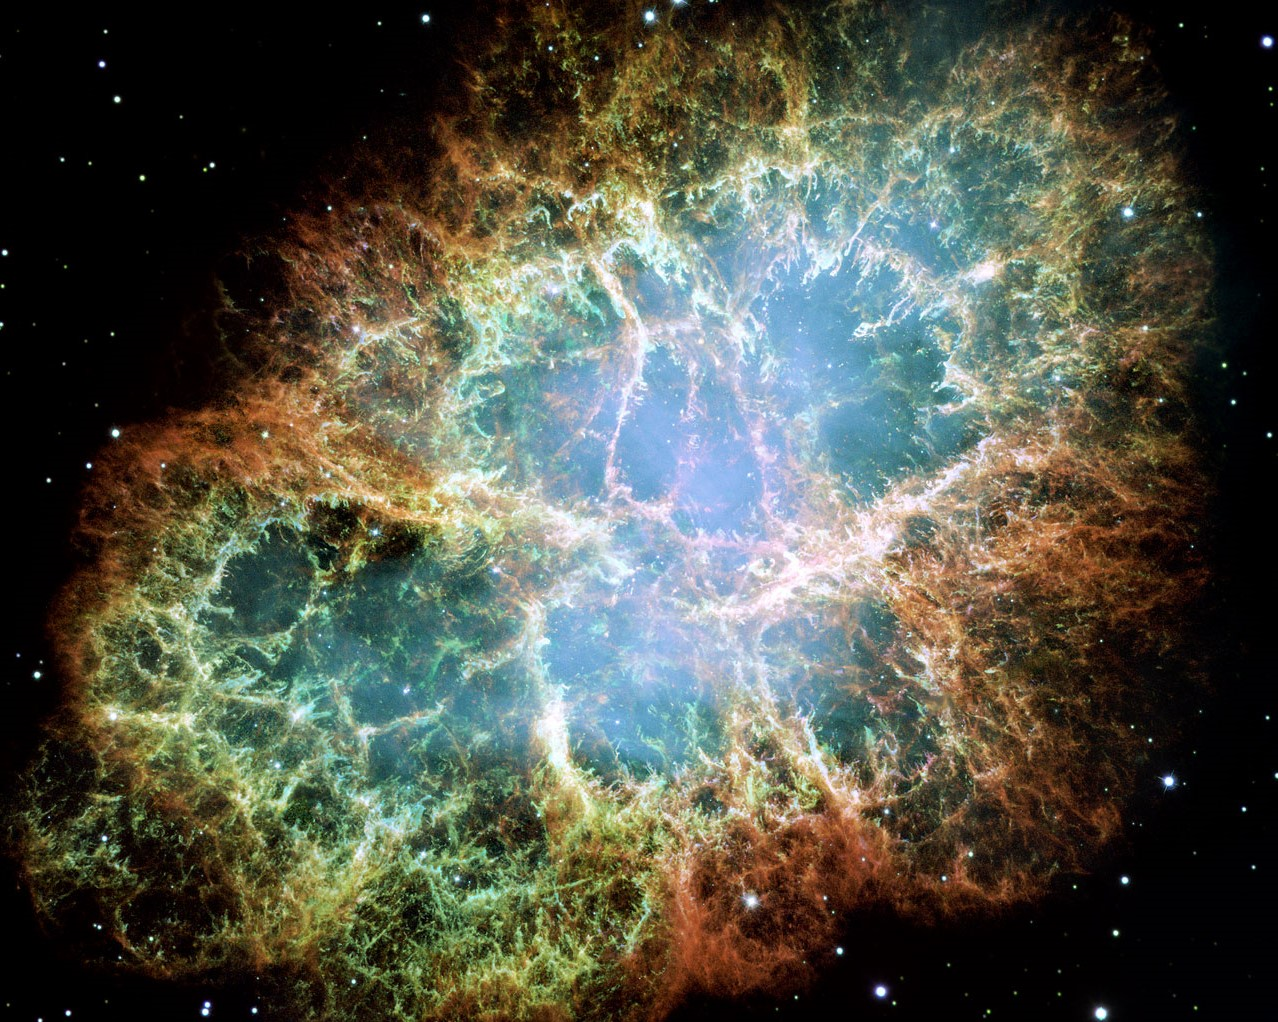
\includegraphics[width=\paperwidth, height =10cm]{../Crab.jpg}}
    \end{figure}
\end{titlepage}

%%%%%%%%%%%%%%%%%%%%%%%
\tableofcontents


%%%%%%%%%%%%%%%%%%%%%%%%%%%%%%%%%%%%% Part 1
\part{The Real Numbers: StillWell}

%%%%%%%%%%%%%%%%%%%%%% Chapter 1.1
\chapter{Ordinals}

\section{Counting Past Infinity}

The sets involved in our infinite counting process are called \textbf{ordinal numbers}, or simply \textbf{ordinals}. The natural numbers are represented by the \textbf{finite ordinals}. The finite ordinals are defined as follows: \begin{align*}
    0 &:= \emptyset \\
    1 &:= 0\cup \{0\} \\
    2 &:= 1\cup \{1\} \\
    &\vdots
\end{align*}
With this each finite ordinal is the set of all its predecessors, and $m < n$ if and only if $m \in n$. Then we take the first infinite ordinal to be \begin{equation*}
    \omega = \bigcup_nn = \{0,1,2,3,...\}
\end{equation*}
This is the right choice, but it requires the assumption of existence of infinite sets.

Recall an \textbf{isolated point} of a closed set $F$ is a point $P \in F$ with an $\varepsilon$-neighborhood containing no other points of $F$, and that a closed set $F$ is \textbf{perfect} if it has no isolated points. This suggests we can obtain a perfect subset (if it exists) of a closed set by repeatedly removing isolated points. This involves taking the derived set, $F'$, possibly ad-infinum. In 1872 this led Cantor to develop the theory of ordinals to count ``past the finite numbers."


\section{What are Ordinals?}


Von Neumann (1923) was the first to provide a definition of ordinal numbers as a particular kind of set. 


\subsection{Finite Ordinals}

The number $0$ is defined to be the empty set, $\emptyset$. Then $1,2,3,...$ are constructed as described previously. Note we gain a connection between number theory and set theory:
\begin{itemize}
    \item For any natural numbers $m$ and $n$, $m < n \iff m \in n$
    \item The successor function $S(n) = n\cup \{n\}$
\end{itemize}

\subsection{Infinite Ordinals: Successor and Least Upper Bound}

To define infinite ordinals we refine the key idea of the previous section: an ordinal is the set of all its predecessors. We can say $\omega$ is the least infinite ordinal because its predecessors are all the finite ordinals. We can also say that $\omega$ is the least upper bound of the finite ordinals. Thus the step from finite to infinite ordinals demands the existence of the infinite set $\omega$. 

The successor operation $S(x) = x\cup \{x\}$ applies to any set. So, starting with $\omega$ we can generate an infinite sequence of infinite ordinals, $\omega+1,\omega+2,\omega+3,...$. Then bracing them all together we obtain their least upper bound \begin{equation*}
    \omega\cdot 2 = \{0,1,2,...,\omega,\omega+1,\omega+2,...\}
\end{equation*}
Another sequence of successors then leads to $\omega\cdot 3,\omega \cdot 4,...$.

The sequence of ordinals $\omega,\omega\cdot 2,\omega\cdot 3,...$ also has a least upper bound, which we obtain by collecting all of these sets, and all their predecessors, into a single set $\omega^2$. This is simply the union of $\omega,\omega\cdot 2,\omega\cdot 3,...$. In this way we can grasp ordinals $\omega^3,\omega^4,...$ and their least upper bound $\omega^{\omega}$, then ordinals $\omega^{\omega^2},\omega^{\omega^3},\omega^{\omega^4},...$, and their least upper bound $\omega^{\omega^{\omega}}$ and so on.

Note that we have still not left the realm of countable ordinals.

\subsection{Uncountable Ordinals}

The least uncountable ordinal, $\omega_1$, should be the set of all countable ordinals. However to make this precise we need a precise definition of ordinal and $<$.

\begin{defn}
    An \textbf{ordinal} $\alpha$ is a set that is \begin{itemize}
        \item $\in$-transitive: that is, if $\beta \in \alpha$ and $\gamma \in \beta$, then $\gamma \in \alpha$
        \item $\in$-linear: that is, $\beta,\gamma \in \alpha$, then either $\beta \in \gamma$ or $\gamma \in \beta$
    \end{itemize}
    Also $\beta < \alpha$ if and only if $\beta\in \alpha$.
\end{defn}


We more fully encorporate the axioms of set theory later, but for now we iterate a key axiom for this approach: the \textbf{axiom of foundation}, which says that there is no infinite descending membership sequence $\cdots \in \alpha_3\ in \alpha_2 \in \alpha_1$. The axiom of foundation ensures that each set of ordinals has a least member, and hence it enables definitions and proofs by induction on ordinals, i.e. transfinite induction.


\section{Well-Ordering and Transfinite Induction}

The usual statement of the \textbf{Axiom of Foundation} is 
\begin{defn}[Axiom of Foundation]
    Each nonempty set $S$ has an $\in$-least member; that is, an element $x \in S$ such that $y \notin x$ for any $y \in S$.
\end{defn}

It follows, in particular, that $x \notin x$ for any set $x$, and the definition of ordinal implies that any ordinal is \textbf{linearly ordered} by the membership relation $\in$. That is, if we write the usual order symbol$ <$ in place of $\in$, then any $\alpha,\beta,\gamma$ in $\sigma$ satisfy \begin{itemize}
    \item[1.] $\alpha \nless \alpha$
    \item[2.] If $\alpha \neq \beta$, then either $\alpha < \beta$ or $\beta < \alpha$
    \item[3.] If $\alpha < \beta$ and $\beta < \gamma$, then $\alpha < \gamma$
\end{itemize}
The axiom of foundation gives a fourth property making the linear ordering a well-ordering: 
\begin{itemize}
    \item[4.] Any subset of $\sigma$ has a least member.
\end{itemize}

Ordinals are not the only well-ordered sets, but they include the order types of all well-ordered sets, in the following sense: 
\begin{thm}[Ordinal Representation of Well-orderings]
    If $<$ is a well-ordering relation on a set $W$, then $(W,<)$ is order isomorphic to some ordinal $\sigma$ under the relation $\in$. That is there is a bijection $f:\sigma\rightarrow W$ such that $$\alpha \in \beta \iff f(\alpha) < f(\beta)$$
\end{thm}
\begin{proof}
    We would like to define $f$ ``inductively" by saying $f(0) = $ least member of $W$, and $f(\alpha) = $ least member of $W-\{f(\beta):\beta <\alpha\}$ until we reach an ordinal $\sigma$ such that $\{f(\beta):\beta < \sigma\}  = W$. However we have not yet proved this approach is valid.

    Instead consider all bijections $f_{\alpha}$ between ordinals $\alpha$ and subsets of $W$, satisfying the following: \begin{itemize}
        \item[1.] $f_{\alpha}(\beta)$ is defined for all $\beta < \alpha$
        \item[2.] $f_{\alpha}(0) = $ least member of $W$.
        \item[3.] For any $\gamma < \alpha, f_{\alpha}(\gamma) = $ least member of $W-\{f_{\alpha}(\beta):\beta < \gamma\}$
    \end{itemize}
    The set of such functions is not empty since it includes the function $f_1$ consisting of a single ordered pair $(0, $ least member of $W)$.
    Also any two such functions, say $f_{\alpha}$ and $g_{\delta}$, are compatible in the sense that they agree on all ordinals for which they are both defined.

    Now let $\sigma$ be the least ordinal greater than all the $\alpha$ for which $f_{\alpha}$ exists. By compatibility, $\{f_{\alpha}:\alpha < \sigma\}$ is an injection $f:\sigma\rightarrow W$. If $f$ is not onto then $W-\{f(\alpha):\alpha < \sigma\}$ is not empty, and we can define \begin{equation*}
        f(\sigma) = \text{ least member of }W - \{f(\alpha):\alpha < \sigma\}
    \end{equation*}
    which contradicts the definition of $\sigma$.

    Thus $f$ is a bijection, and it follows from conditions $2$ and $3$ that $f$ is order-preserving.
\end{proof}


\begin{cor}
    For any two ordinals $\mu$ and $\nu$, either $\mu \in \nu$ or $\nu \in \mu$.
\end{cor}



\section{The Cantor-Bendixson Theorem}

In the following we use the term \textbf{limit} for an ordinal that is not a successor.

\begin{defn}
    If $F$ is a closed set, then $F^{(\alpha)}$ is defined for all countable ordinals $\alpha$ as follows (the $\alpha$-th derived set): \begin{align*}
        F^{(1)} &= F-\{\text{all isolated points of }F\} \\
        F^{(\alpha+1)} &= F^{(\alpha)} - \{\text{all isolated points of }F^{(\alpha)}\} \\
        F^{(\lambda)} &= \bigcap_{\alpha < \lambda}F^{(\alpha)} \;\;\text{ when $\lambda$ is a limit ordinal} 
    \end{align*}
\end{defn}

In a construction like this where points are removed at successor stages, taking the intersection is natural at a limit stage because it omits all the points removed from $F^{(\alpha)}$ at all stages $\alpha+1 < \lambda$. This sequence becomes constant at some countable ordinal $\alpha$.

\begin{lem}
    If we have open sets $U_{\alpha}$ for $\alpha \leq$ some ordinal $\gamma$, and if $\alpha < \beta \leq \gamma$ implies $U_{\alpha} \subsetneq U_{\beta}$, then $\gamma$ is countable.
\end{lem}
\begin{proof}
    Since $U_{\alpha} \subsetneq U_{\alpha+1}$, for each $\alpha < \gamma$ we have a point $x_{\alpha} \in U_{\alpha+1}-U_{\alpha}$ and hence a rational open interval $I_{\alpha}$ such that $x_{\alpha} \in I_{\alpha} \subseteq U_{\alpha+1}$. Indeed we can define $I_{\alpha}$ explicitly as the first interval $I$ (in some fixed enumeration of the rational intervals) such that $I \subseteq U_{\alpha+1}$ but $I \nsubset U_{\alpha}$.

    The intervals $I_{\alpha},I_{\beta}$ are necessarily different for $\alpha < \beta$, since $I_{\alpha} \subset U_{\beta}$ but $I_{\beta} \nsubset U_{\beta}$, hence there are only countable many ordinals $< \gamma$, because there are only countable many rational intervals.
\end{proof}


\begin{thm}[Cantor-Bendixson Theorem]
    If $F$ is a closed subset of $\R$ and $F^{(\alpha)}$ denotes the $\alpha$th derived set of $F$, then $F^{(\alpha)} = F^{(\alpha+1)}$ for some countable $\alpha$, and hence $F^{(\alpha)}$ is either empty or perfect.
\end{thm}
\begin{proof}
    It follows from the definition of the sets $F^{(\alpha)}$ that they are all closed and that $F_{\alpha} \supseteq F_{\beta}$ for $\alpha < \beta$. Hence the open complements $U_{\alpha}$ of the $F^{(\alpha)}$ are such that $U_{\alpha} \subseteq U_{\beta}$ for $\alpha < \beta$.

    Then since a nested well-ordered sequence of open sets has countable length, it follows that $U_{\alpha} = U_{\alpha+1}$ for some countable ordinal $\alpha$, and hence $F^{(\alpha)} = F^{(\alpha+1)}$.
\end{proof}



\section{The ZF Axioms for Set Theory}

In this section we list the most commonly used axioms for set theory, which are the \textbf{Zermelo-Fraenkel Axioms}, after Ernst Zermelo who proposed most of them in 1908, and Abraham Fraenkel who made an important amendment in 1922.

The underlying idea of the ZF axioms is that ``everything is a set". Then all relations between sets are based on membership and equality. We also require a formal logic to base our set theory on, which we do not cover in these notes. Most ZF axioms describe operations for producing new sets from old. Implicitly, they describe the cumulative concept of set, according to which each set is constructed from previously defined sets (starting with the empty set). Thus sets arise in stages, which turn out to be ordinal number stages.


\textbf{Axioms of ZF}:
\begin{itemize}
    \item \textbf{Extensionality.} Two sets are equal if and only if they have the same members. That is \begin{equation*}
            \forall A\forall B(A=B\iff \forall x(x \in A\iff x \in B))
    \end{equation*}
    \item \textbf{Empty Set.} There is a set with no members. \begin{equation*}
            \exists \emptyset\forall x(\lnot x \in \emptyset)
    \end{equation*}
    \item \textbf{Pairing.} For any sets $X$ and $Y$, there is a set $\{X,Y\}$ whose only members are $X$ and $Y$. \begin{equation*}
        \forall X \forall Y\exists Z\forall T(T \in Z\iff (T = X\lor T = Y))
    \end{equation*}
        The pairing axiom gives us the \textbf{unordered pair} $\{X,Y\}$, but we can also get the \textbf{ordered pair} $\langle X,Y\rangle$, namely \begin{equation*}
            \langle X,Y\rangle = \{\{X\},\{X,Y\}\}
        \end{equation*}
    \item \textbf{Union.} For any set $X$ there is a set whose members are the members of members of $X$. \begin{equation*}
            \forall X\exists U\forall Y(Y \in U \iff \exists T(T \in X \land Y \in T))
    \end{equation*}
    \item \textbf{Infinity.} There is an infinite set; in fact a set that includes $0$ and, along with any member $X$, also the member $X \cup \{X\}$. \begin{equation*}
            \exists N(\emptyset \in N \land \forall X(X \in N\implies X\cup \{X\} \in N))
    \end{equation*}
    \item \textbf{Replacement.} For any function definition $f$, the values $f(x)$, where $x$ is a member of a set $X$ (the domain of $f$), form a set $f(X)$ (the range of $f$). \begin{equation*}
            \forall X\forall Y\forall (f:X\rightarrow Y)\exists U\forall y(y \in U \iff \exists x(x \in X\land f(x) = y))
    \end{equation*}
        This is actually an infinite schema of axioms, one for each two-variable formula $\varphi(x,y)$ written in the language of ZF. Such a formula defines a function $f$ if, for each $x \in X$, $\varphi(x,y)$ holds for exactly one $y$.
    \item \textbf{Power Set.} For any set $X$ there is a set $\mathcal{P}(X)$ whose members are the subsets of $X$. $\mathcal{P}(X)$ is called the \textbf{power set} of $X$. \begin{equation*}
            \forall X\exists Y\forall Z(Z \in Y \iff \forall x(x \in Z\implies x \in X))
    \end{equation*}
    \item \textbf{Foundation.} Every set $X$ has a $\in$-minimal member; that is, an $x \in X$ such that $y \in x$ for no $y \in X$. \begin{equation*}
            \forall X\exists x\forall y(y \in X\implies \lnot y \in x)
    \end{equation*}
        This implies that Foundation guarantees that any set that is linearly ordered by the membership relation $\in$ is in fact well-ordered by $\in$, which simplifies the definition of ordinal. Foundation also guarantees the cumulative set concept, by ensuring that each set $X$ has a rank $\alpha$- an ordinal number that counts the number of applications of the power set axiom needed to build $X$, starting from the empty set.
\end{itemize}



\section{Finite Set Theory and Arithmetic}

As we saw previously the numbers $0,1,2,3,...$ can be taken to be the sets $0 = \emptyset, 1 = \{0\},2 = \{0,1\},...$, with the successor function $S(n) = n\cup \{n\}$. Thus ZF can prove the existence of the basic objects of arithmetic. In fact, if we omit Infinity from the ZF axioms, the remaining axiom set ZF$-$Infinity is equivalent to the Grassmann-Dedekind-Peano axioms. Note the axiom of foundation gives us definition and proof by induction.

In detail, here is how the foundations of arithmetic can be established in ZF$-$Infinity:
\begin{enumerate}
    \item The natural numbers $0,1,2,3,...$ are the finite ordinals. An ordinal $\alpha$ is finite if $\alpha$ and all of its members each have a greatest member, where $\gamma$ is the greatest member of $\beta$ if $\gamma \in \beta$ and $\gamma \notin \delta$ for any $\delta \in \beta$.
    \item Induction amounts to the principle that, if some natural number $n$ has property $P$, then there is a least natural number with property $P$ (for properties $P$ definable in the language of ZF). Since $n$ is a finite ordinal, the numbers $\leq n$ are the members of $S(n) = n \cup \{n\}$, so the least member with property $P$ is the least member of the set \begin{equation*}
            \{m:m \in n\cup \{n\}\text{ and $m$ has property $P$}\}
    \end{equation*}
        This least member exists by the foundation axiom.
    \item Since induction is available, we can define sum and product as before.
\end{enumerate}

The only sets that ZF$-$Infinity can prove to exist are those obtained from the empty set $0$ by iterating the power set operation a finite number of times. We can encode these finite sets by natural numbers and set operations such as pairing and union by operations on numbers, so in this way arithmetic is ``equivalent" to ZF$-$Infinity.

\section{The Rank Hierarchy}

\begin{defn}
    Sets $V_{\alpha}$ are defined as follows for ordinals $\alpha$: \begin{itemize}
        \item $V_0 = 0$ (the empty set)
        \item $V_{\alpha+1}= \mathcal{P}(V_{\alpha})$ \\
        \item $V_{\lambda} = \bigcup_{\beta < \lambda}V_{\beta}$ for each limit ordinal $\lambda$
    \end{itemize}
    The \textbf{rank} of a set $X$ is defined inductively as the least $\alpha$ such that each member of $X$ has rank less than $\alpha$.
\end{defn}

Thus $V_{\alpha}$ may be viewed as the set of all sets built using $< \alpha$ applications of the power seet operation $\mathcal{P}$, and the claim that every set is built at some stage is: 

\begin{thm}[Existence of Rank] 
    Each set $X$ has a rank.
\end{thm}
\begin{proof}
    Suppose $X$ is a set that does not have a rank. Then some member $_1$ of $X$ also does not have a rank, Because if each $x \in X$ has a rank, $\text{rank}(x)$, the replacement axiom tells us that the range of the rank function on $X$ is a set of ordinals, with union $\alpha$ say. This means that $X$ has a rank $(\leq \alpha+1)$, contrary to assumption.

    Thus there are members $X_1$ with no rank, and similarly members $X_2$ of these $X_1$ with no rank, and so on. With the help of the replacement and union axioms we can collect these into a single set $N$. But then $N$ is a set with no $\in$-minimal member, contrary to the foundation axiom.
\end{proof}

The universe of all sets can be viewed as the union of the sets $V_{\alpha}$, as $\alpha$ ranges over all the ordinals. We denote this by $V$, though $V$ is not a set.


\subsection{Cardinality}

\begin{defn}
    For any set $X$, let $\alpha$ be the minimal rank of a set with the same cardinality as $X$. Then the \textbf{cardinality of $X$} is the set \begin{equation*}
        \{Y \in V_{\alpha}:Y\text{ has the same cardinality as $X$}\}
    \end{equation*}
\end{defn}


\section{Large Sets}

\begin{defn}
    A set is \textbf{inaccessible} if it has infinite members and is closed under the operations of power set and taking ranges of functions.
\end{defn}

If $V_{\alpha}$ is an inacessible set, then $V_{\alpha}$ satisfies the ZF axioms. Certainly if $V_{\alpha}$ is large enough to have an infinite member, then it satisfies the empty set and infinity axioms. Closure under power set also guarantees that $\alpha$ is a limit ordinal, in which case $V_{\alpha}$ is also closed under pairing and union, so $V_{\alpha}$ satisfies the pairing and union axioms. Finally $V_{\alpha}$ satisfies foundation, so $V_{\alpha}$ satisfies all the ZF axioms.

Now suppose we take the least $\alpha$ such that $V_{\alpha}$ is inaccessible. It follows that any $V_{\beta}$ in $V_{\alpha}$ is not inaccessible, so $V_{\alpha}$ satisfies the sentence ``there is no inacessible $V_{\beta}$". Existence of an inaccessible set is therefore not provable in ZF.

It is actually in the nature of strong axiom systems like ZF that there are many sentences they can state but neither prove nor disprove. Such sentences are said to be \textbf{independent} of the system in question. The famous incompleteness theorem of G\"{o}del gives a general explanation for this phenomenon of independent sentences.

It should be mentioned that for any ``sufficiently strong" axiom system $\sum$, there is a sentence $\text{Con}(\sum)$ expressing the consistency of $\sum$, which is independent of $\sum$ if $\sum$ is consistent. This is \textbf{G\"{o}del's second incompleteness theorem}. Because of this, statements about consistency of strong systems take a relative form: ``if $\sum$ is consistent then so is $\Omega$".

For example results of G\"{o}del show ``If ZF is consistent, then so is ZF$+$AC$+$CH". 






%%%%%%%%%%%%%%%%%%%%%% Chapter 1.2
\chapter{Axiom of Choice}


\section{Some Naive Questions about Infinity}

In the early days of set theory the following questions arose:

\begin{enumerate}
    \item Does every infinite set have a countably infinite subset?
        The naive answer is yes, because if $S$ is infinite we can remove an element $s_1$ from $S$, and $S-\{s_1\}$ is still infinite. Then we can remove an element $s_2$ from $S-\{s_1\}$ and $S-\{s_1,s_2\}$ is still infinite, and so on. But this requires a countable number of arbitrary ``choices"
    \item Is a countable union of countable sets countable?

        Again the naive answer is yes, via a diagonal arrangement: \begin{align*}
            S_1 &= \{s_{11},s_{12},s_{13},...\} \\
            S_2 &= \{s_{21},s_{22},s_{23},...\} \\
            S_3 &= \{s_{31},s_{32},s_{33},...\}  \\
            &\vdots
        \end{align*}
        Then we can enumerate the members by members of $\N\times \N$, so $S_1\cup S_2\cup \cdots $ is countable
    \item If a function $f$ is sequentially continuous at $x$, is $f$ continuous at $x$?

        Again a countable choice of points within $1/2^n$ of $x$.
\end{enumerate}

In the three examples above we have a commonality of an infinite sequence of choices, with choices coming with no apparent definition\---one just has to believe that it exists. So far this is countable choice. Zermelo introduced the following stronger version:

\begin{defn}[Axiom of Choice]
    If $X$ is any set whose members are nonempty, then there exists a function $F$, called a \textbf{choice function for $X$}, such that $F(x) \in x$ for each $x \in X$.
\end{defn}

Thus, the function $F$ ``chooses" a member $F(x)$ from each member $x$ of $X$. Here is how we deploy it in the above examples:

\begin{enumerate}
    \item Let $X$ be the set of all nonempty subsets of the given infinite set $S$, and let $F$ be a choice function for $X$. Then we can define the sequence $\langle s_1,s_2,...\rangle$ inductively in terms of $F$: \begin{equation*}
            s_1 = F(S),\;s_n = F(S-\{s_1,s_2,...,s_{n-1}\})
    \end{equation*}
    \item Let $E(S_i)$ be the set of all enumerations of the countably infinite set $S_i$, let $X = \{E(S_i):i \in \N\}$, and let $F$ be a choice function for $X$. Then we can define the enumeration $\{s_{i1},s_{i2},...\}$ of $S_i$ as $F(E(S_i))$ and complete the proof as before.
    \item Our assumption is that in any open interval $I$ that contains $x$ there exists an $x'$ with $|f(x')-f(x)| \geq \varepsilon_0$. We therefore have, for each $n$, a nonempty set $$J_n = \{x':|x'-x| < 1/2^n\text{ and }|f(x')-f(x)|\geq \varepsilon_0\}$$
        We define $X = \{J_1,J_2,...\}$ and let $F$ be a choice function for $X$. Then $x_n' = F(J_n)$ has the property $$|x'_n - x| < 1/2^n\;\text{ and }\;|f(x'_n)-f(x)| \geq \varepsilon_0$$
        as required.
\end{enumerate}
In the latter two cases we are using the so-called \textbf{countable choice axiom}, where choices are made from each member of a countable set. In the first case we use the so-called \textbf{dependent choice axiom}, where a sequence of choices is made, each dependent on the one before.


\section{The Full Axiom of Choice and Well-Ordering}


We have the following theorem of Zermelo:

\begin{thm}[Well-Ordering Theorem]
    Assuming the full axiom of choice, there is a bijection between any set $X$ and an ordinal.
\end{thm}
\begin{proof}[Sketch]
    The basic idea is to repeatedly choose elements $x_0,x_1,x_2,...$ from $X$, assigning them ordinal numbers as subscripts. When all the ordinals less than $\alpha$ have been assigned, the next element chosen is assigned subscript $\alpha$. Since any set of ordinals has a least upper bound $\alpha$, we can continue assigning ordinals to members of $X$ until $X$ is exhausted. This gives a bijection between $X$ and some ordinal $\alpha$ (the least upper bound of the ordinals assigned to members of $X$)
\end{proof}

\begin{proof}
    Let $F$ be a choice function for the nonempty subsets of $X$. $F$ enables us to define the following function $g$, mapping ordinals into $X$, by induction: $$g(0) = x_0 = F(X)$$
    and if $g(\beta)$ has been defined for $\beta < \alpha$, let $$g(\alpha) = x_{\alpha} = F(X-\{x_{\beta}:\beta < \alpha\})$$
    To see each member of $X$ equals $x_{\beta}$ for some ordinal $\beta$, consider the members of $X$ that are of the form $g(\beta)$. These form a subset $S$ of $X$, and hence \begin{equation*}
        \{\beta:g(\beta)\text{ is defined}\} = g^{-1}(S)
    \end{equation*}
    is a set of ordinals, by the replacement schema. But this set has an upper bound $\alpha$, since any set of ordinals has a least upper bound. Hence $g(\alpha) = x_{\alpha}$ is defined, unless the elements $x_{\beta}$, for $\beta < \alpha$, include all elements of $X$.
     
     Since $g(\alpha)$ is not defined, by definition, it follows that $S = X$, and that $g$ is a bijection between $X$ and the ordinal $\alpha$.
\end{proof}

This theorem is called the well-ordering theorem because it says that any set can be ordered like the ordinal numbers, which are well-ordered by the $<$ relation. Well-ordering carries over to any set $X$ if we label its elements with ordinal numbers as subscripts and then order its elements by the relation $\prec$ defined by $$x_{\alpha} \prec x_{\beta} \iff \alpha < \beta$$

This means we can employ a well-ordering of $\R$, but we only know it exists, we cannot describe it. Its elusiveness is indicative of the elusiveness of sets obtained from the axiom of choice. It cannot be less elusive because well-ordering of every set implies the axiom of choice.

\begin{thm}[Well-ordering implies the axiom of choice]
    If every set has a well-ordering, then every set has a choice function.
\end{thm}
\begin{proof}
    Given a set $X$ whose members are nonempty sets, we find a choice function for $X$ as follows. Let $Y$ be the union of all members $x$ of $X$, and take a well-ordering $\prec$ of $Y$. Then each $x$ is a subset of $Y$, well-ordered by the relation $\prec$. So the function defined by \begin{equation*}
        F(x) = (\prec-\text{least member of }x)
    \end{equation*}
    is a choice function for $X$.
\end{proof}


\subsection{Cardinal Numbers}

The well-ordering theorem allows us to define the \textbf{cardinal number} of each set simply. Assuming AC, each set is equinumerous with an ordinal by the well-ordering theorem, and so we can make the definition $$|X| = \text{cardinal number of $X$} = \text{least ordinal equinumerous with $X$}$$
For example, $|\N| = \omega$, and $|\{\text{countable ordinals}\}| = \omega_1$. When talking about cardinal numbers it is usual to use alephs: $\aleph_0 = \omega,\aleph_1 = \omega_1$, and so on. This notation is useful as there is a sense of \textbf{cardinal arithmetic} (reflecting size) different from ordinal arithmetic (reflecting order). In ordinal arithmetic we have $$\omega+\omega = \omega\cdot 2 \neq \omega$$ but in cardinal arithmetic we have $$\aleph_0+\aleph_0 = \aleph_0$$
to reflect the fact that the union of two disjoint countably infinite sets is countably infinite. Similarly, $$\omega\cdot \omega = \omega^2 \neq \omega\;\text{ but }\;\aleph_0\cdot\aleph_0 = \aleph_0$$



\section{The Continuum Hypothesis}

Cantor formulated the \textbf{continuum hypothesis}, which originally stated simply that every uncountable set of real numbers has the same cardinality as $\R$. Then after developing his theory of ordinal numbers and well-ordered sets, he hoped that $\R$ could be well-ordered, and further that $\R$ had the smallest uncountable cardinality, $\aleph_1$. This is what the continuum hypothesis means today:

\begin{defn}[Continuum Hypothesis]
    There is a bijection between $\R$ and the least uncountable ordinal, $\omega_1$.
\end{defn}

In the language of cardinal arithmetic: $2^{\aleph_0} = \aleph_1$. In the absence of plausible new axioms, AC can only guarantee the existence of a well-ordering of $\R$; it cannot name any such ordering. It so happens that there is an axiom, called the \textbf{axiom of constructibility}, which provides a definable well-ordering of every set and is consistent with the ZF axioms. This was introduced by G\"{o}del and it gives a definition of each set in a language $\mathcal{L}$ that includes the symbols of the ZF language plus symbols for all the ordinals. THe sets named by $\mathcal{L}$ are called the \textbf{constructible sets}. The axiom of constructibility states that every set is constructible, and this axiom is consistent with ZF because $\mathcal{L}$ gives names for enough sets to satisfy the ZF axioms. Moreover, it is possible to define a well-ordering of all the formulas in $\mathcal{L}$, and hence of all the constructible sets. 

Moreover, it turns out that each real number in $L$ is defined by a formula in $\mathcal{L}$ involving only symbols for countable ordinals, so the real numbers in $L$ can be ordered in a sequence of length $\omega_1$, and hence $L$ satisfies the continuum hypothesis. Although a definable well-ordering may be good for the universe, it is not necessarily good for $\R$. The definable well-ordering of $\R$ implied by the axiom of constructibility implies that there are definable subsets of $\R$ with bizarre properties.


\section{Filters and Ultrafilters}

The lowest level theorems for which an axiom of choice may be required are those about sets of natural numbers. In this section we give an example\---the existence of a nonprincipal ultrafilter over $\N$.

\begin{defn}
    A collection $\mathcal{F}$ of subsets of a set is called a \textbf{filter} if \begin{enumerate}
        \item $\emptyset \notin \mathcal{F}$
        \item If $A \in \mathcal{F}$ and $A \subseteq B$, then $B \in \mathcal{F}$
        \item If $A,B \in \mathcal{F}$ then $A\cap B \in \mathcal{F}$
    \end{enumerate}
\end{defn}
In other words a filter is a collection of subsets that does not include the empty set and is closed under supersets and intersections.

\begin{eg}
    For any $a \in \N$, $\mathcal{F}_a = \{A \subseteq \N:a \in A\}$ is a filter. $\mathcal{F}_a$ is called the \textbf{principal filter} generated by $a$.

    The set of \textbf{cofinite subsets} of $\N$, $\{X \subseteq \N:\N-X\text{ is finite}\}$ is a filter
\end{eg}

The principal filter above satisfies an additional condition making it an \textbf{ultrafilter}: \begin{enumerate}
    \item[4.] For each subset $B$, either $B \in \mathcal{F}$ or $B^c \in \mathcal{F}$.
\end{enumerate}

This raises the question: are there any nonprincipal ultrafilters over $\N$? One way to answer this is if we are able to extend the filter of cofinite sets to an ultrafilter, since no $a \in \N$ can be in all cofinite sets. This involves applying the following a possibly uncountable number of times.

\begin{thm}[Filter Extension]
    If $\mathcal{F}$ is a filter over $X$ that is not an ultrafilter\---so both $A \notin \mathcal{F}$ and $A^c\notin \mathcal{F}$ for some $A$\---then there is a filter $\mathcal{H}\supset \mathcal{F}$ with $A \in \mathcal{H}$.
\end{thm}
\begin{proof}
    We extend the set $\mathcal{F}$ to $\mathcal{H}$ in two stages that ensure closure of $\mathcal{H}$ under intersections and supersets: 
    \begin{itemize}
        \item[Stage 1.] Add to $\mathcal{F}$ all sets of the form $A\cap F$, where $F \in \mathcal{F}$. The resulting set $$\mathcal{G} = \mathcal{F} \cup \{A\cap F:F \in \mathcal{F}\}$$
            is closed under intersections.
        \item[Stage 2.] Add all supersets $B \supseteq A\cap F$ of the sets added at stage 1. Since the supersets of each $F \in \mathcal{F}$ were already in $\mathcal{F}$ the resulting set \begin{equation*}
                \mathcal{H} = \mathcal{F} \cup \{B \supseteq A\cap F:F \in \mathcal{F}\}
        \end{equation*}
            is closed under supersets.
    \end{itemize}
    Finally, we observe that the empty set $\emptyset \notin \mathcal{H}$ because the elements of $\mathcal{H}$ are supersets of sets of the form $F$ or $A\cap F$, where $F \in \mathcal{F}$. We know that each $F \neq \emptyset$ because $\mathcal{F}$ is a filter. And if $A\cap F = \emptyset$, then $F \subseteq X-A$, which implies $X-A \in \mathcal{F}$, contrary to assumption.
\end{proof}

With the axiom of choice we can carry out this process infinitely until we obtain an ultrafilter.

\begin{thm}[Extension to an ultrafilter]
    Any filter over $X\neq \emptyset$ is contained in an ultrafilter over $X$.
\end{thm}
\begin{proof}
    Given a filter $\mathcal{F}$ over $X$ we build an increasing sequence of filters $\mathcal{F}_{\alpha}$ whose union is an ultrafilter. To define the $\mathcal{F}_{\alpha}$ we use AC to obtain a well-ordering $A_0,A_1,...,A_{\alpha}$, for $\alpha < \lambda$, of all subsets of $X$. Then we let \begin{align*}
        \mathcal{F}_0 &= \mathcal{F} \\
        \mathcal{F}_{\alpha+1} &= \left\{\begin{array}{cc} \mathcal{F}_{\alpha}\text{ if }A_{\alpha} \in \mathcal{F}_{\alpha}\text{ or }X-A_{\alpha} \in \mathcal{F}_{\alpha} \\ \text{extension of }\mathcal{F}_{\alpha}\text{ by }A_{\alpha}\text{ otherwise} \end{array}\right. \\
        \mathcal{F}_{\beta} &= \bigcup_{\gamma < \beta}\mathcal{F}_{\gamma}\text{ for each limit ordinal $\beta$}
    \end{align*}
    It follows by filter extension that $\mathcal{F}_{\alpha+1}$ is a filter when $\mathcal{F}_{\alpha}$ is. It is also clear that $\bigcup_{\gamma < \beta}\mathcal{F}_{\gamma}$ is a filter when each$\mathcal{F}_{\gamma}$ is.

    Thus, it follows by transfinite induction that $\mathcal{F}_{\alpha}$ is a filter for each $\alpha$, and $\mathcal{F}_{\lambda}$ is also a filter by the argument for limit ordinals. Finally, either $A_{\alpha} \in \mathcal{F}_{\lambda}$ or $X-A_{\alpha} \in \mathcal{F}_{\lambda}$ for each $\alpha$, by construction, so $\mathcal{F}_{\lambda}$ is an ultrafilter that extends $\mathcal{F}$ (\textbf{This last bit may only apply for the case of $X = \N$}).
\end{proof}


\section{Games and Winning Strategies}

Our next application of AC is in the theory of infinite games. Consider two-person games in which players I and II move alternately and there is a bound on the length of complete sequences of moves. Such a game is called finite, and it is said to be with \textbf{perfect information} if each player knows all previous moves. In any such game one of the players may have a winning strategy; that is, a rule for making moves that always leads to a win. In tic-tac-toe neither player has a winning strategy, but if drawing ended in a win for some player then one would.

\begin{thm}[Winning strategy theorem]
    If $\mathcal{G}$ is a finite two-person game with perfect information, in which every play ends in a win for one of the players, then either player $I$ or player $II$ has a winning strategy.
\end{thm}
\begin{proof}
    Since the game $\mathcal{G}$ is finite, all possible plays of $\mathcal{G}$ can be captured as paths in a tree with Start vertex, and vertices immediately below representing the positions that can be reached by the first move. Since $\mathcal{G}$ is finite, there is a maximum value $N$ for the length of downward branches from the start vertex.

    We prove a winning strategy by induction on $N$. If $N = 1$ then the game ends in one move, and by the hypothesis, every move leads to a win for eithe $I$ or $II$. If any move leads to a win for $I$, then choosing that move is a winning strategy for $I$. If every move leads to a win for $II$, then letting $I$ make any move is a winning strategy for $II$.

    Now for the induction step, suppose that either $I$ or $II$ has a winning strategy for any game of length $< N$. Among such games are the subgames of $\mathcal{G}$ whose starting positions are the vertices $1,2,...$ in the tree of plays of $\mathcal{G}$. Thus each of the latter games has a winning strategy for either $I$ or $II$.

    But then $I$ or $II$ has a winning strategy for $\mathcal{G}$ itself. If any of the games with starting position $1,2,...$ has a winning strategy for $I$, then $I$ has a winning strategy for $\mathcal{G}$. It consists of making their first move into such a subgame, $n$ say, and thereafter playing a winning strategy for the game $n$. If none of the games has a winning strategy for $I$, then they all have winning strategies for $II$, in which case $II$ has a winning strategy for $\mathcal{G}$. 
\end{proof}



\section{Infinite Games}

If we remove the restriction that all plays in a game have length bounded by some integer $N$, and if we allow each move to be chosen from some countable set, then the finite tree now represents all possible plays in a countably infinite game with prefect information. Each play is given by an infinite sequence $\langle a_1,b_1,a_2,b_2,...\rangle$ where $a_1,a_2,a_3,...$ represent the successive moves by player $I$ and $b_1,b_2,b_3,...$ represent the successive moves by player $II$. The game itself is defined by a set $X$ of such sequences; namely those that represent a win for player $I$. We call this game $\mathcal{G}_X$. Thus in $\mathcal{G}_X$ player $I$ tries to ensure that the sequence $\langle a_1,b_1,a_2,b_2,...\rangle \in X$, while $II$ tries to ensure that $\langle a_1,b_1,a_2,b_2,...\rangle \notin X$.

It was conjectured by Steinhaus that in such games one player has a winning strategy, as in the finite case, but the AC makes it possible to define a set $X$ for which neither player has a winning strategy. Such a set $X$ is called \textbf{undetermined}.

\subsection{Strategies}

In any game $\mathcal{G}_X$, a \textbf{play} is a sequence $\langle a_1,b_1,a_2,b_2,...\rangle$. A \textbf{strategy} $\sigma$ is a positive integer-valued function defined on all finite sequences of positive integers, including the empty sequence. Player $I$ plays strategy $\sigma$ by making the moves \begin{align*}
    a_1 &= \sigma(\langle\rangle) \\
    a_2 &= \sigma(\langle b_1\rangle) \\
    a_3 &= \sigma(\langle b_1,b_2\rangle) \\
    &\vdots 
\end{align*}
in response to moves made by player $II$. Player $II$ plays strategy $\sigma$ by making moves \begin{align*}
    b_1 &= \sigma(\langle a_1\rangle) \\
    b_2 &= \sigma(\langle a_1,a_2\rangle) \\
    b_3 &= \sigma(\langle a_1,a_2,a_3\rangle) \\
    &\vdots 
\end{align*}
in response to moves made by player $I$.

We let $\sigma*b$ denote the play that results when $I$ plays strategy $\sigma$ on the sequence $b$ of moves made by player $II$. And we say that $\sigma$ is a \textbf{winning strategy for $I$} in the game $\mathcal{G}_A$ if $\sigma*b \in A$ for all sequences of moves $b$ by player $II$. Similary, we let $a*\sigma$ denote the play that results when $II$ plays strategy $\sigma$ on the sequence $a$ of moves made by player $I$, and we say that $\sigma$ is a \textbf{winning strategy} for $II$ in game $\mathcal{G}_A$ if $a*\sigma \notin A$ for all sequences $a$.

The set of strategies $\sigma$ has cardinality $2^{\aleph_0}$ (same as $\N^{\N}$).

\begin{thm}[An undetermined set]
    There exists a set $X \subset \N^{\N}$ for which neither player has a winning strategy for the game $\mathcal{G}_X$.
\end{thm}
\begin{proof}
    Let $\{\sigma_{\alpha}:\alpha < 2^{\aleph_0}\}$ be an enumeration of all strategies. Using this enumeration, we will inductively choose the members of disjoint subsets of $\N^{\N}$, \begin{equation*}
        X = \{x_{\alpha}:\alpha < 2^{\aleph_0}\}\text{  and  }Y = \{y_{\alpha}:\alpha < 2^{\aleph_0}\}
    \end{equation*}
    Each $x_{\alpha}$ witnesses the fact that $\sigma_{\alpha}$ is not a winning strategy for $II$ in the game $\mathcal{G}_X$, because we will arrange that $a*\sigma_{\alpha} = x_{\alpha} \in X$ for some $a \in \N^{\N}$. Each $y_{\alpha}$ will witness the fact that $\sigma_{\alpha}$ is not a winning strategy for $I$ either, because we will arrange that $\sigma_{\alpha}*b = y_{\alpha} \notin X$ for some $b \in \N^{\N}$.

    At stage $0$ we make these arrangements, and keep $x_0$ and $y_0$ in disjoint sets, by letting \begin{align*}
        x_0 &= \text{any value of }a*\sigma_0 \\
        y_0 &= \text{any value of }\sigma_0*b\text{ unequal to $x_0$}
    \end{align*}
    Such a value $y_0$ exists because $\sigma_0*b$ takes $2^{\aleph_0}$ values as $b$ runs through $\N^{\N}$, since $b$ consists of all the even-numbered places in $\sigma_0*b$.


    At stage $\alpha$ less than $2^{\aleph_0}$ values $x_{\beta},y_{\beta}$ have yet been chosen, so enough values $a*\sigma_{\alpha}$ and $\sigma_{\alpha}*b$ remain to let \begin{align*}
        x_{\alpha} &= \text{any value of }a*\sigma_{\alpha}\text{ not in }\{y_{\beta}:\beta < \alpha\} \\
        y_{\alpha} &= \text{any value of }\sigma_{\alpha}*b\text{ not in }\{x_{\beta}:\beta \leq \alpha\}
    \end{align*}
    It follows by induction on $\alpha$ that $X$ and $Y$ have no common member, and for each $\alpha < 2^{\aleph_0}$ we have witnesses to the fact that $\sigma_{\alpha}$ is not a winning strategy for either $II$ or $I$ in the game $\mathcal{G}_X$. Since $\sigma_{\alpha}$ exhaust all strategies, it follows that the set $X$ is undetermined.
\end{proof}


\section{The Countable Axiom of Choice}

We now consider the special case of the axiom of choice, the \textbf{countable axiom of choice}:

\begin{defn}[Countable AC]
    Any countable set $\{\mathcal{S}_1,\mathcal{S}_2,\mathcal{S}_3,...\}$ of nonempty sets $\mathcal{S}_n$ has a choice function; that is, a function $f$ such that $f(\mathcal{S}_n) \in \mathcal{S}_n$ for each $n$.
\end{defn}

Countable AC is useful and in fact necessary to prove some basic theorems of analysis, like the third example appearing in the first section of this chapter. As full AC causes some irregularities in the theory of $\R$ it is useful to restrict when we can to weaker versions like countable AC.

An interesting candidate axiom for one which implies countable AC but not AC is the \textbf{axiom of determinacy}, AD.

\begin{defn}[Axiom of Determinacy]
    For any set $X \subset \N^{\N}$, either player $I$ or player $II$ has a winning strategy for the game $\mathcal{G}_X$.
\end{defn}

\begin{thm}[AD implies countable AC for subsets of $\N^{\N}$]
    Given a countable set $\mathcal{S} = \{S_1,S_2,S_3,...\}$, where each $S_n \subset \N^{\N}$, AD gives a choice function for $\mathcal{S}$
\end{thm}
\begin{proof}
    Given a countable set $\{S_1,S_2,S_3,...\}$ of sets $S_n \subset \N^{\N}$, consider the following game. If $I$ plays $\langle a_1,a_2,...\rangle \in \N^{\N}$ and $II$ plays $\langle b_1,b_2,...\rangle \N^{\N}$, then $II$ wins if and only if $\langle b_1,b_2,...\rangle \in S_{a_1}$. This game can be formulated as $\mathcal{G}_X$ for a certain $X \subset \N^{\N}$, namely $$X = \{\langle a_1,b_1,a_2,b_2,...\rangle:\langle b_1,b_2,...\rangle \notin S_{a_1}\}$$
    Therefore, AD says that either $I$ or $II$ has a winning strategy.

    Now player $I$ does not have a winning strategy for this game, because after $I$ plays $a_1$ player $II$ can always win by playing some $\langle b_1,b_2,...\rangle$ in the nonempty set $S_{a_1}$. So player $II$ has a winning strategy; that is, a function $f$ which, among other things, for each $a_1$ gives a $\langle b_1,b_2,b_3,...\rangle \in S_{a_1}$. In other words, a winning strategy for $II$ gives a choice function for the sets $S_1,S_2,...$.
\end{proof}

This tells us that although AD is incompatible with full AC, it actually implies enough choice for some important applications to analysis.


\section{Zorn's Lemma}

Many books construct ultrafilters by a method of Zorn's Lemma instead of transfinite induction.

\begin{defn}[Zorn's Lemma]
    Suppose that $\mathcal{T}$ is a set such that each linearly ordered subset $\mathcal{S}$ has an upper bound: that is, an $X \in \mathcal{T}$ such that $Y \leq X$ for each $Y \in \mathcal{S}$. Then $\mathcal{T}$ has a maximal element; that is a $Z \in \mathcal{T}$ such that $Z \leq Y$ ofr any $Y \in \mathcal{T}$ implies $Z = Y$.
\end{defn}

We mainly apply this when the partial order $\leq$ is set inclusion.

\begin{thm}[Extension to an Ultrafilter]
    Any filter over $X$ is contained in an ultrafilter over $X$.
\end{thm}
\begin{proof}
    Let $\mathcal{T}$ be the set of all filters over $X$. If $\mathcal{S}$ is a set of filters that is linearly ordered by set inclusion, then the union $X$ of all filters in $\mathcal{S}$ is itself a filter. Thus $\mathcal{T}$ satisfies the condition of Zorn's lemma, and hence $\mathcal{T}$ has a maximal element $Z$. In other words, $Z$ is a filter over $X$ that is not properly contained in any other filter. This implies $Z$ is an ultrafilter, otherwise it could be extended by the filter extension theorem.
\end{proof}

It turns out that in ZF, Zorn's lemma is equivalent to AC, as we now prove.

\begin{thm}[Equivalence Theorem]
    In ZF, Zorn's lemma is equivalent to AC.
\end{thm}
\begin{proof}
    We first suppose AC. Suppose we are given a set $\mathcal{T}$ in which each linearly ordered subset $\mathcal{S}$ has an upper bound. AC gives a function such that $$f(\mathcal{S}) = \text{ an upper bound of }\mathcal{S}$$
    for each $\mathcal{S} \subseteq \mathcal{T}$ that is linearly ordered by $\subseteq$. Morevoer, we can stipulate that $$f(\mathcal{S})\supsetneq \text{ each element of }\mathcal{S}$$
    if such an element exists. Using the function $f$, and transfinite induction, we define a linearly ordered sequence of sets $A_{\alpha} \in \mathcal{T}$ whose upper bound is necessarily maximal, namely, let \begin{align*}
        A_0 &=\text{ any element of }\mathcal{T} \\
        A_{\alpha} &= f(\mathcal{T}-\{f(\beta):\beta < \alpha\}) 
    \end{align*}
    The $A_{\alpha}$ form a set, by the replacement axiom, since $\alpha$ cannot exceed the cardinality of $\mathcal{T}$. The set $A_{\alpha}$ is linearly ordered, by transfinite induction. And its upper bound is maximal by definition of $f$, since $f$ always chooses an element greater than any chosen earlier, if it can. 


    Conversely, if Zorn's lemma holds, we can obtain a well-ordering of any set $X$ (and hence AC) as follows. Consider the set $\mathcal{T}$ of all bijections between subsets of $X$ and ordinals. Such a bijection, $$g:Y\rightarrow \alpha$$ is of course a set of ordered pairs, and if $g_1 \subset g_2$ then $g_2$ extends $g_1$ from a subset $Y_1 \subseteq X$ to a larger subset $Y_2 \subseteq X$, by agreeing with $g_1$ on $Y_1$ and mapping the members of $Y_2 - Y_1$ to larger ordinals.

    So if we have a set $\mathcal{S}$ of these bijections, linearly ordered by inclusion, its union will itself be such a bijection, and hence an upper bound of $\mathcal{S}$ in $\mathcal{T}$. Thus, $\mathcal{T}$ satisfies the conditions of Zorn's lemma, which then gives a maximal element of $\mathcal{T}$. That is a bijection $g$ between a subset $Y \subseteq X$ and an ordinal $\alpha$ that cannot be extended. It follows that $Y = X$, because if $x \in X-Y$ we can extend $g:Y\rightarrow \alpha$ by the ordered pair $\langle x,\alpha\rangle$) and hence $g$ gives a well-ordering of $X$.
\end{proof}





%%%%%%%%%%%%%%%%%%%%%% - Appendices
\begin{appendices}
	

\end{appendices}


\end{document}


%%%%%% END %%%%%%%%%%%%%
